 \documentclass{article}

%% Packages %%
\usepackage[utf8]{inputenc}
\usepackage{amssymb, amsthm, tabto, epigraph, mathtools, physics, dsfont, verbatim, slashed, mathrsfs}
\usepackage{graphicx, wrapfig}
\usepackage[shortlabels]{enumitem}
\usepackage{relsize}
\usepackage{subcaption}
\usepackage{csquotes}
\usepackage{hyperref}
\usepackage{todonotes}
\usepackage{braket}
\usepackage{tikz}
\usepackage{faktor}
\usepackage{tensor}
\usepackage{cancel}

%% Configure some Packages %%
\setlist{nolistsep}
\hypersetup{
    colorlinks=true,
    linkcolor=black,
    filecolor=magenta,      
    urlcolor=blue,
}

\usepackage[
backend=biber,
sorting=none,
style=numeric-comp
]{biblatex}
\addbibresource{references.bib}

%% Coloured Text for Draft and Editing %%
\usepackage{xcolor}
\newcommand{\ques}[1]{\textcolor{red}{#1}}
\newcommand{\ans}[1]{\textcolor{blue}{#1}}

%% Math operators %%
\DeclareMathOperator{\Hom}{Hom}
\DeclareMathOperator{\Ker}{Ker}
\DeclareMathOperator{\im}{Im}
\DeclareMathOperator{\Tor}{Tor}
\DeclareMathOperator{\Pf}{Pf}
\newcommand{\Mod}[1]{\ (\mathrm{mod}\ #1)}
\DeclareMathOperator{\mfT}{\mathfrak{T}}
\DeclareMathOperator{\bbZ}{\mathbb{Z}}
\DeclareMathOperator{\bbR}{\mathbb{R}}
\DeclareMathOperator{\bbC}{\mathbb{C}}
\DeclareMathOperator{\id}{\mathds{1}}
\DeclareMathOperator{\Arf}{\textrm{Arf}}
\DeclareMathOperator{\diag}{\textrm{diag}}
 
\newtheorem{theorem}{Theorem}

%% Subdirectory Access %%
\graphicspath{{./images/}}

\title{Duality Defects in \texorpdfstring{$E_8$}{E8}}
\author{}
\date{}

\begin{document}

\maketitle
\tableofcontents

\vskip 1cm
\noindent \textbf{To do}:
\begin{enumerate}
    \item asd
\end{enumerate}

\newpage

\section{Introduction}

\subsection{The \texorpdfstring{$E_8$}{E8} Lattice}

\begin{figure}
    \centering
    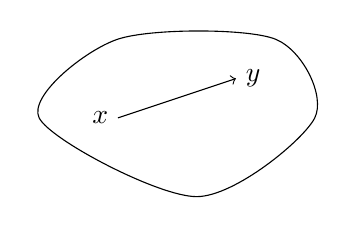
\begin{tikzpicture}
    \draw plot [smooth cycle] coordinates {(0,0) (1,1) (3,1) (3.5,0) (2,-1)};
    \draw [->] (1,0) node [anchor = east] {$x$} -- (2.5,0.5) node [anchor = west] {$y$};
    \end{tikzpicture}
    \caption{A convex set. All of the points in the line containing $x$ and $y$ lie in this set.}
\end{figure}

We will focus on the lattice $E_8$ of vectors $l\in\mathbb{R}^8$ such that either
\begin{enumerate}
    \item $l\in\mathbb{Z}^8$ and $\sum_{i=1}^8l^i\in 2\mathbb{Z}$, or
    \item $l\in(\mathbb{Z}+1/2)^8$ and $\sum_{i=1}^8l^i\in 2\mathbb{Z}+1$.
\end{enumerate}
This lattice is even, in that for all $l\in E_8$ we have $\langle l,l\rangle\in2\mathbb{Z}$. Thus, its roots are given by all vectors $l\in E_8$ with $\langle l,l\rangle=2$. Choosing a vector $n\in\mathbb{R}^8\setminus\{0\}$ gives an orientation to it's orthogonal hyperplane. If such a hyperplane does not intersect any elements of $E_8$, it separates the lattice points into positive and negative. Explicitly, we say that $l\in\mathbb{R}^8$ is positive (negative) if $\langle l, n\rangle>0$ ($\langle l,n\rangle<0$). Choosing, for example, $n=(1.1,1.2,1.3,1.4,1.5,1.6,1.7,1.8)$, we find that the lattice can be described as the set of integer linear combinations
\begin{equation}
    E_8=\mathbb{Z}\alpha_1\oplus\cdots\oplus\mathbb{Z}\alpha_8
\end{equation}
of the basis of positive roots
\begin{equation}
    \begin{aligned}
    \alpha_1&=(-1,1,0,\dots,0)\\
    \alpha_2&=(0,-1,1,0,\dots,0)\\
    \vdots&\\
    \alpha_7 & = (0,\dots,0,-1,1)\\
    \alpha_8 &=(1/2,1/2,1/2,1/2,1/2,-1/2,-1/2,-1/2).
    \end{aligned}
\end{equation}
With these we can build the Cartan matrix
\begin{equation}
C_{ij}=\cancel{2}\frac{\langle \alpha_i,\alpha_j\rangle}{\cancel{\langle \alpha_j,\alpha_j\rangle}}=\mqty(2&-1 &0 &0 &0 &0 &0 &0\\
-1 &2 &-1 &0 &0 &0 &0 &0\\
0& -1 &2 &-1 &0 &0 &0 &0\\
0 &0&-1 &2 &-1 &0 &0 &0 \\
0 &0&0&-1 &2 &-1 &0 &-1 \\
0 &0&0& 0&-1 &2 &-1 &0 \\
0&0&0&0 &0&-1 &2 &0\\
0 &0&0 &0 &-1 &0 &0 &2)_{ij}
\end{equation}
which is succinctly encoded into the (compact) Dynkin diagram
\begin{equation}
    \begin{tikzpicture}
    \draw (1,0) node [anchor = west] {$\alpha_1$};
    \draw (1.6,0) -- (2.1,0) node [anchor = west] {$\alpha_2$};
    \draw (2.7,0) -- (3.2,0) node [anchor = west] {$\alpha_3$};
    \draw (3.8,0) -- (4.3,0) node [anchor = west] {$\alpha_4$};
    \draw (4.9,0) -- (5.4,0) node [anchor = west] {$\alpha_5$};
    \draw (6,0) -- (6.5,0) node [anchor = west] {$\alpha_6$};
    \draw (7.1,0) -- (7.6,0) node [anchor = west] {$\alpha_7$.};
    \draw (5.7,0.3) -- (5.7,0.8) node [anchor = south] {$\alpha_8$}; 
    \end{tikzpicture}
\end{equation}
In here, each line between each vector encodes that they have the same length and there is an angle of $\pi/3$ between them. Moreover, one can also check that the highest root from the hyperplane orthogonal to $n$ is given by
\begin{equation}
\alpha_{\textrm{high}}=2\alpha_1+3\alpha_2+4\alpha_3+5\alpha_4+6\alpha_5++ 4\alpha_6+2\alpha_7+3\alpha_8.
\end{equation}
By computing the inner products $\langle\alpha_{\textrm{high}},\alpha_i\rangle$ one sees that this vector fits into the extended (affine) Dynkin diagram
\begin{equation}\label{eq:affine_E_8}
    \begin{tikzpicture}
    \draw (0,0) node {$\alpha_{\text{high}}$};
    \draw (0.5,0) -- (1,0) node [anchor = west] {$\alpha_1$};
    \draw (1.6,0) -- (2.1,0) node [anchor = west] {$\alpha_2$};
    \draw (2.7,0) -- (3.2,0) node [anchor = west] {$\alpha_3$};
    \draw (3.8,0) -- (4.3,0) node [anchor = west] {$\alpha_4$};
    \draw (4.9,0) -- (5.4,0) node [anchor = west] {$\alpha_5$};
    \draw (6,0) -- (6.5,0) node [anchor = west] {$\alpha_6$};
    \draw (7.1,0) -- (7.6,0) node [anchor = west] {$\alpha_7$.};
    \draw (5.7,0.3) -- (5.7,0.8) node [anchor = south] {$\alpha_8$}; 
    \end{tikzpicture}
\end{equation}
For computations, it is useful to introduce the dual basis $(\omega_1,\dots,\omega_8)$, for which $\langle\omega_i,\alpha_j\rangle=\delta_{ij}$. The matrix of inner products of these is quickly obtained by inverting our Cartan matrix
\begin{equation}
\langle\omega_i,\omega_j\rangle=\mqty(2 & 3 & 4 & 5 & 6 & 4 & 2 & 3\\
3 & 6 & 8 &10 &12 & 8 & 4 & 6\\
4 & 8 &12 &15 &18 &12 & 6 & 9\\
5 &10 &15 &20 &24 &16 & 8 &12\\
6 &12 &18 &24 &30 &20 &10 &15\\
4 & 8 &12 &16 &20 &14 & 7 &10\\
2 & 4 & 6 & 8 &10 & 7 & 4 & 5\\
3 & 6 & 9 &12 &15 &10 & 5 & 8\\)_{ij}.
\end{equation}

\subsection{The Vertex Operator Algebra \texorpdfstring{$V_{E_8}$}{VE8}}

Let us consider the theory of a closed string moving in the torus $\faktor{\mathbb{R}^8}{E_8}$. A vibrationless state of the string is described by its winding around this torus. Thus, for every $l\in E_8$ we have a string state $\ket{l}$ obtained by taking an open string in $\mathbb{R}^8$ starting at $0$ and ending at $l$, and then winding it into a closed string in our torus $\faktor{\mathbb{R}^8}{E_8}$. In particular, we have the vacuum state which consists of a vibrationless state without winding $\ket{0}$. For every $l\in E_8$ we associate an operator which creates the associated winding
\begin{equation}
\Gamma_{l}\ket{0}=\ket{l}.
\end{equation}
We must thus have that for every $l_1,l_2\in E_8$ then $\Gamma_{l_1}\Gamma_{l_2}\propto\Gamma_{l_1+l_2}$. Asking for $\Gamma$ to be a representation of the lattice won't allow us to construct local fields in general. We must then content ourselves with projective representations. Therefore $\Gamma_{l_1}\Gamma_{l_2}=\epsilon(l_1,l_2)\Gamma_{l_1+l_2}$, with $\epsilon(v,l)\in\mathbb{C}\setminus\{0\}$. The associativity of the action of these winding operators guarantees that for $l_1,l_2,l_3$ we have
\begin{equation}
\begin{aligned}
\epsilon(l_1,l_2)\epsilon(l_1+l_2,l_3)\ket{l_1+l_2+l_3}&=(\Gamma_{l_1}\Gamma_{l_2})\ket{l_3}=\Gamma_{l_1}(\Gamma_{l_2}\ket{l_3})\\
&=\epsilon(l_1,l_2+l_3)\epsilon(l_2,l_3)\ket{l_1+l_2+l_3},
\end{aligned}
\end{equation}
i.e. $\epsilon(l_1,l_2)\epsilon(l_1+l_2,l_3)=\epsilon(l_1,l_2+l_3)\epsilon(l_2,l_3)$. In terms of group cohomology, this means that $\epsilon$ is a 2-cocycle. We can in fact always take $\epsilon(l_1,l_2)\in\{\pm1\}$, i.e. the 2-cocycle in the trivial $E_8$ module $\mathbb{Z}_2$. We can in fact also choose the convention
\begin{equation}
\epsilon(l,l)=(-1)^{\langle l,l\rangle}.
\end{equation} 
More importantly however, we will see that we will need to require that $\epsilon(l_1,l_2)=(-1)^{\langle l_1,l_2\rangle}\epsilon(l_2,l_1)$. This determines $\epsilon$ up to a 2-coboundary. The algebra generated by the operators $\Set{\Gamma_l|l\in E_8}$ is called the twisted group algebra $\mathbb{C}_\epsilon(E_8)$.

This theory also has a set of operators $\Set{a_n^{(i)}|n\in\mathbb{Z}\text{ and }i\in\{1,\dots,8\}}$, which create the $n$th vibrational mode of the string in the $i$th direction. These satisfy the commutation relations
\begin{equation}
[\alpha_n^{(i)},\alpha_m^{(j)}]=m\delta_{m+n,0}\delta^{ij}.
\end{equation}
The Lie algebra generated by these operators and $1\in\mathbb{C}$ is known as the Heisenberg algebra.\todo{I decided to omit the placeholder $\vb{k}$ for $1$ to make it look more familiar to physicists.} The operators with $n\geq 0$ act as annihilation operators for the vacuum state $a_n^{(i)}\ket{0}=0$. Those with $n=0$ act trivially $a_0^{(i)}\ket{0}=0$. We complete our description of the operators of our theory by imposing the following commutation relations between the twisted group algebra and the Heisenberg algebra
\begin{equation}
\begin{aligned}
[a_n^{(i)},\Gamma_l]&=0,\qquad n\neq 0\\
[a_0^{(i)},\Gamma_l]&=l^i.
\end{aligned}
\end{equation}
These in particular act on the Fock space $V_{E_8}$, spanned by a basis 
\begin{equation}
\{a_{n_1}^{(i_1)}\cdots a_{n_k}^{(i_k)}\ket{l}|n_1,\dots,n_k\in\mathbb{Z}^-\textrm{, }i_1,\dots,i_k\in\{1,\dots,8\}\textrm{, and }l\in E_8\}.
\end{equation}
$V_{E_8}$ is graded if to each of the elements of the basis above we assign a degree given by the number of vibrational modes it has and the length of its winding
\begin{equation}
n_1+\cdots+n_k+\langle l,l\rangle/2.
\end{equation}

\section{\texorpdfstring{$E_8$}{E8} and Non-Anomalous Symmetries}

\subsection{Gauging Symmetries of \texorpdfstring{$E_8$}{E8}}

\todo{$V_{E_8}$ vs $VE_8$?}

The symmetries of $V_{E_8}$i up to conjugacy, are determined by vectors $x\in\mathbb{R}^8$ satisfying
\begin{enumerate}
    \item $\langle\alpha_i,x\rangle\geq 0$ for all $i\in\{1,\dots,8\}$ and
    \item $\langle\alpha_{\text{high}},x\rangle\leq 1$. 
\end{enumerate}
The corresponding symmetry acts trivially on the Heisenberg module and through phases on the twisted group algebra
\begin{equation}
    \begin{aligned}
    \ket{0}&\mapsto\ket{0},\\
    a_n^{(i)}&\mapsto a_n^{(i)},\\
    \Gamma_l&\mapsto e^{2\pi i\ev{x,l}}\Gamma_l.
    \end{aligned}
\end{equation}
Notice then that we obtain a $\mathbb{Z}_N$ symmetry if and only if $N$ is the smallest positive integer for which $N\langle x,l\rangle\in\mathbb{Z}$. 

The gauging of a symmetry described by such a vector $x$, consists of first understanding the invariant gauge operators. These correspond to the VOA $V_{E_8^x}$ of the lattice
\begin{equation}
    E_8^x=\Set{l\in E_8|\langle l,x\rangle\in\mathbb{Z}}.
\end{equation}
This, however, is in general not self-dual. Therefore, the corresponding VOA does not describe an holomorphic CFT. Thus, as a second step in the gauging procedure, we extend the invariant algebra to the VOA corresponding to a self-dual extension of $E_8^x$ different from our original $E_8$. If such an extension exists, it is unique. If such an extension does not exist, we say that $x$ describes an anomalous symmetry.

Let us describe briefly the technique for finding such an extension $\Lambda$. Let us begin by assuming that it exists. Then, since both $\Lambda$ and $E_8$ are self-dual lattices containing $E_8^x$, we have
\begin{equation}
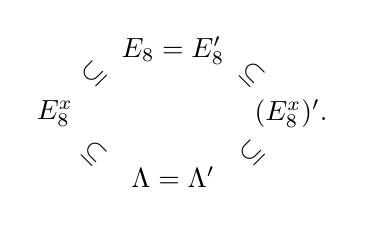
\begin{tikzpicture}
\node at (-1,0) {$E_8^x$};
\node at (-0.5,0.5) {\rotatebox{45}{$\subseteq$}};
\node at (-0.5,-0.5) {\rotatebox{-45}{$\subseteq$}};
\node at (0.5,0.8) {$E_8=E_8'$};
\node at (0.5,-0.8) {$\Lambda=\Lambda'$};
\node at (1.5,-0.5) {\rotatebox{45}{$\subseteq$}};
\node at (1.5,0.5) {\rotatebox{-45}{$\subseteq$}};
\node at (2,0) {$(E_8^x)'$.};
\end{tikzpicture}
\end{equation}
Therefore, $\Lambda$ can be constructed by  the cosets of $E_8^x$ inside of $(E_8^x)'$. The space $\faktor{(E_8^x)'}{E_8^x}$ of these contains, in particular, $E_8^x$ and the cosets in $\faktor{E_8}{E_8^x}$. Of course, to build $\Lambda$, one needs to make sure that $E_8^x\in\faktor{\Lambda}{E_8^x}$. Moreover, self-dual lattices cannot be further extended. Indeed, if $L_1\subseteq L_2$ are both selfdual, then $L_1\subseteq L_2=(L_2)'\subseteq(L_1)'=L_1$. Thus, $\faktor{\Lambda}{E_8^x}$ must not contain all of the cosets in $ \faktor{E_8}{E_8^x}$ and must contain at least one coset in $\faktor{(E_8^x)'}{E_8^x}$ that is not in $\faktor{E_8}{E_8^x}$.

\subsection{Case Study: \texorpdfstring{$\mathbb{Z}_2$}{Z2} Symmetries}

To see an explicit example of the ideas developed above, let us consider the $\mathbb{Z}_2$ symmetries of $V_{E_8}$. Being of order $2$, they are described by vectors $x\in\mathbb{R}^8$ such that $2x\in(E_8)'$. Thus, $2x$ is an integer linear combination of the basis $(\omega_1,\dots,\omega_8)$. In fact, due to the requirement that $\langle \alpha_i,x\rangle\geq 0$, the linear combination must consist entirely of positive numbers. We can then see that the condition $\langle x,\alpha_{\text{high}}\rangle\leq 1$ shows that there are only two $\mathbb{Z}_2$ symmetries described by $x_1:=\frac{1}{2}\omega_2$ and $x_2:=\frac{1}{2}\omega_7$.

Let us begin by considering the symmetry described by $x_1$. Following the first step of the gauging procedure, we see
\begin{equation}
    \begin{aligned}
    E_8^{x_1}&=\Set{l\in E_8|\langle x_1,l\rangle\in\mathbb{Z}}=\Set{l=\sum_{i=1}^8l_i\alpha_i\in E_8|l_2\in2\mathbb{Z}}\\
    &=\mathbb{Z}\alpha_1\oplus\mathbb{Z}2\alpha_2\oplus\mathbb{Z}\alpha_3\oplus\cdots\oplus\mathbb{Z}\alpha_8.
\end{aligned}
\end{equation}
Then
\begin{equation}
    E_8^{x_1}=\mathbb{Z}\omega_1\oplus\mathbb{Z}\frac{1}{2}\omega_2\oplus\mathbb{Z}\omega_3\oplus\cdots\oplus\mathbb{Z}\omega_8,
\end{equation}
and we can compute the quotient
\begin{equation}
    \faktor{(E_8^{x_1})'}{E_8^{x_1}}=\{E_8^{x_1},\beta_1+E_8^{x_1},\beta_2+E_8^{x_1},\beta_1+\beta_2+E_8^{x_1}\},
\end{equation}
where
\begin{equation}
    \begin{aligned}
    \beta_1&=-\omega_1-\frac{1}{2}\omega_2+\omega_7+\omega_8,\\
    \beta_2&=-\frac{1}{2}\omega_2+\omega_8.
    \end{aligned}
\end{equation}
Now, notice that $|E_8:E_8^{x_1}|=2$. This can be seen by comparing the volumes of their primitive cells
\begin{equation}
    \text{Vol}(E_8^{x_1})=\det(\alpha_1,2\alpha_2,\alpha_3,\dots,\alpha_8)=2\det(\alpha_1,\dots,\alpha_8)=2\text{Vol}(E_8).
\end{equation}
Moreover, $\beta_1+\beta_2=-\omega_1+\omega_2+\omega_7+\omega_8\in (E_8)'=E_8$. We conclude that
\begin{equation}
    \faktor{E_8}{E_8^{x_1}}=\{E_8^{x_1},\beta_1+\beta_2+E_8^{x_1}\}.
\end{equation}
On the other hand, $\langle\beta_1,\beta_1\rangle,\langle\beta_2,\beta_2\rangle\not\in2\mathbb{Z}$. Therefore, none of the other two cosets can be used to extend $E_8^{x_1}$ into another self dual lattice. We conclude that $x_1$ describes an anomalous symmetry.

Let us now consider the symmetry described by the $x_2$. Repeating the same procedure as for the anomalous symmetry, we obtain
\begin{equation}
    E_8^{x_2}=\mathbb{Z}\alpha_1\oplus\cdots\oplus\mathbb{Z}\alpha_6\oplus\mathbb{Z}2\alpha_7\oplus\mathbb{Z}\alpha_8,
\end{equation}
and
\begin{equation}
    \faktor{(E_8^{x_2})'}{E_8^{x_2}}=\{E_8^{x_2},\beta_1+E_8^{x_2},\beta_2+E_8^{x_2},\beta_1+\beta_2+E_8^{x_2}\},
\end{equation}
where now $\beta_1=\frac{1}{2}\omega_7$ and $\beta_2=\omega_8$. As before, we can reconstruct our original lattice
\begin{equation}
    \faktor{E_8}{E_8^{x_2}}=\{E_8^{x_2},\beta_2+E_8^{x_2}\}.
\end{equation}
However, now we have $\langle\beta_1+\beta_2,\beta_1+\beta_2\rangle=14\in2\mathbb{Z}$. Then, we can in fact obtain another self-dual extension 
\begin{equation}
    \faktor{\Lambda}{E_8^{x_2}}=\{E_8^{x_2},\beta_1+\beta_2+E_8^{x_2}\}.
\end{equation}
Thus, $x_2$ describes a non-anomalous symmetry of $V_{E_8}$. For completeness, we remark that the last coset is fermionic since $\langle \beta_1,\beta_1\rangle=1$\todo{Again, what does it mean for a coset to be fermionic?}. In particular, it cannot be used to extend $E_8^{x_2}$ in a self-dual manner.


Finally, we remark that $E_8^{x_2}$ is isomorphic to the $D_8$ lattice. To see this, recall that the highest root fits into the Dynkin diagram as shown in \eqref{eq:affine_E_8}. Moreover, we can equivalently describe
\begin{equation}
    E_8^{x_2}=\mathbb{Z}\alpha_1\oplus\cdots\oplus\mathbb{Z}\alpha_6\oplus\mathbb{Z}\alpha_{\text{high}}\oplus\mathbb{Z}\alpha_8.
\end{equation}
Thus, this lattice is obtained by replacing the root $\alpha_7$ with $\alpha_{\text{high}}$. We conclude that it is described by the Dynkin diagram
\begin{equation}
    \begin{tikzpicture}
    \draw (0,0) node {$\alpha_{\text{high}}$};
    \draw (0.5,0) -- (1,0) node [anchor = west] {$\alpha_1$};
    \draw (1.6,0) -- (2.1,0) node [anchor = west] {$\alpha_2$};
    \draw (2.7,0) -- (3.2,0) node [anchor = west] {$\alpha_3$};
    \draw (3.8,0) -- (4.3,0) node [anchor = west] {$\alpha_4$};
    \draw (4.9,0) -- (5.4,0) node [anchor = west] {$\alpha_5$};
    \draw (6,-0.05) -- (6.5,-0.3) node [anchor = north west] {$\alpha_6$.};
    \draw (6,0.05) -- (6.5,0.3) node [anchor = south west] {$\alpha_8$}; 
    \end{tikzpicture}
\end{equation}

\subsection{Non-Anomalous Symmetries of \texorpdfstring{$E_8$}{E8}}\todo{Sections 2.1 and 2.2 should be reversed?}

\subsection{The \texorpdfstring{$VE_8$}{VE8} CFT}
%Consider the unique holomorphic (1+1)d CFT whose left-moving chiral algebra is $VE_8$ and whose right moving chiral algebra is trivial ($c_L = 8$ and $c_R = 0$). We will also denote this CFT as $VE_8$.

\section{\texorpdfstring{$\bbZ_2$}{Z2} Duality Defects}
Given a 2d (non-spin) QFT $T_b$ on $\Sigma$ with a non-anomalous global $G$ symmetry, one can couple the $G$ symmetry to a background $G$-connection. If $G$ is discrete, this connection is necessarily flat and can be represented by a network of  topological line defects. In other words, every global symmetry of the theory implies the existence of topological defect lines. On the contrary, not every line defect implies the existence of a global symmetry. The topological obstructions that cannot be identified with global symmetries are usually called non-invertible line defects since they cannot be inverted under fusion \cite{topDefectLines}. In the following, we consider the former obstructions but we will come back to the non-invertible ones when we consider duality defects.
\vspace{2mm}

The invertible line defects triangulate $\Sigma$ and are labelled by elements of $G$ (see e.g. \cite{generalizedSymmetries}). When a local operator charged under $G$ crosses the topological defect line labelled by $g\in G$, it applies the appropriate (linear) $g$-action to the operator. Intuitively, the lines are labelling the holonomy around a non-contractible loop in $\Sigma$. Viewed this way, a ``twisted partition function'' of a theory is the ``regular'' partition function with choices of these invertible topological defect lines inserted around non-contractible loops.
\vspace{2mm}

Below, we derive the $E_8$ partition function and the $G=\bbZ_2$ twisted partition functions associated with the various insertions of invertible topological defect lines. In this section we will use bozonization and fermionization to find Kramers-Wannier duality defect in $VE_8$ following the techniques of \cite{monsterCFT}, and produce the so-called ``defected partition functions'' associated with inserting these duality defect lines.

\subsection{\texorpdfstring{$E_8$}{E8} Partition Function and \texorpdfstring{$\bbZ_2$}{Z2} Twists}
As stated before we first consider a holomorphic $(1 + 1)$d bosonic CFT theory whose target space is simply $T = \mathcal{R}^8/$L. By definition, the partition function of $VE_8$ is given by
\begin{align}
    Z_{E_8}(\tau)
        &:= \Tr_{\mathcal{H}}(q^{L_0-\frac{c}{24}})\\
        &= \frac{1}{\eta(\tau)^8} \sum_{\lambda \in E_8} q^{\frac{1}{2}\lambda^2}\\
        &= \frac{1}{2\eta(\tau)^8} \left(\theta_1(\tau)^8 + \theta_2(\tau)^8 + \theta_3(\tau)^8 + \theta_4(\tau)^8\right)\\
        &= \frac{1}{q^{1/3}} + 248 q^{2/3} + 4124 q^{5/3} + \dots\,,
\end{align}
where $q=e^{2\pi i \tau}$. Viewing our theory as a chiral boson theory with target $\bbR^8/E_8$, the $\eta$ contributions are interpreted as coming from vibrational modes, and the sum over the $E_8$ lattice as coming from winding sectors. Notice that indeed, the partition function corresponds to a bosonic theory since it has no spin structure associated to it. Moreover we can recognize that it is not invariant under modular $T$ transformations because the theory has $c_L-c_R=8$. In particular, it transforms as $T:Z(\tau) \to e^{-2\pi i/3} Z(\tau)$.
\vspace{2mm}

For simplicity, we will define $Z_{E_8}[0,0] := Z_{E_8}(\tau)$ (suppressing $\tau$), so that we can denote the twisted partition functions for the $\bbZ_2$ orbifold as $Z_{E_8}[g,h]$ where $g,h\in\bbZ_2$. Said differently, $g,h$ are providing the data for a background $\bbZ_2$ connection in $H^1(T^2,\bbZ_2)$.

We recognize this partition functions as being the GSO projection of 16 Majorana-Weyl fermions. In particular, for a single fermion we have that
\begin{align}
    \Tr_{\textrm{NS}} q^{L_0 - \frac{c}{24}} \sim \sqrt{\frac{\theta_3(\tau)}{\eta(\tau)}}\\
    \Tr_{\textrm{R}} q^{L_0 - \frac{c}{24}} \sim \sqrt{\frac{\theta_2(\tau)}{\eta(\tau)}}\\
    \Tr_{\textrm{NS}} (-1)^F q^{L_0 - \frac{c}{24}} \sim \sqrt{\frac{\theta_4(\tau)}{\eta(\tau)}}\\
    \Tr_{\textrm{R}} (-1)^F q^{L_0 - \frac{c}{24}} \sim \sqrt{\frac{\theta_1(\tau)}{\eta(\tau)}}\,,
\end{align}
see, for example, \cite{seibergWitten:spinStructInString}. This fact will be useful later for computing the duality defects of our theory.

From earlier, we know the action of the (non-anomalous) $\bbZ_2$-subgroup on states of our theory. This allows us to compute the twisted partition function for the theory with a topological defect line (called $\eta$ in accordance with \cite{monsterCFT}) inserted along the space direction
\begin{align}
    Z_{E_8}[0,1] 
        &:= \Tr_{\mathcal{H}}( \eta \, q^{L_0-\frac{c}{24}})\\
        &= \frac{1}{2\eta(\tau)^8} \left(\theta_1(\tau)^8 - \theta_2(\tau)^8 + \theta_3(\tau)^8 + \theta_4(\tau)^8\right)\\
        &= \frac{1}{q^{1/3}} - 8 q^{2/3} + 28 q^{5/3} + \dots\,.
\end{align}
Similarly, we have the $\bbZ_2$-generating topological defect line inserted along the time direction
\begin{align}
    Z_{E_8}[1,0]
        &:= \Tr_{\mathcal{H}_\eta}(q^{L_0-\frac{c}{24}})\\
        &= \frac{1}{2\eta(\tau)^8} \left(\theta_1(\tau)^8 + \theta_2(\tau)^8 + \theta_3(\tau)^8 - \theta_4(\tau)^8\right)\\
        &= 16q^{1/6} + 128 q^{2/3} + 576 q^{7/6} + \dots\,.
\end{align}
Likewise, we can insert the $\eta$ topological defect line along both the space and time directions to produce
\begin{align}
    Z_{E_8}[1,1]
        &:= \Tr_{\mathcal{H}_\eta}( \eta \, q^{L_0-\frac{c}{24}})\\
        &= \frac{1}{2\eta(\tau)^8} \left(\theta_1(\tau)^8 + \theta_2(\tau)^8 - \theta_3(\tau)^8 + \theta_4(\tau)^8\right)\\
        &= -16q^{1/6} + 128 q^{2/3} - 576 q^{7/6} + \dots\,.
\end{align}

These partition functions transform correctly into one another under $S$ and $T$ transformations (up to a possible factor of $e^{-2\pi i/3}$). Furthermore, since we know $VE_8$ is the unique holomorphic CFT with $c_L = 8$ and $c_R = 0$, then we can confirm that the $\bbZ_2$-orbifold (gauged theory) has the same partition function
\begin{align}
    Z_{E_8//\bbZ_2}(\tau) 
        &= \frac{1}{2} \sum_{g,h} Z_{E_8}[g,h]\\
        &= \frac{1}{2\eta(\tau)^8} \left(\theta_1(\tau)^8 + \theta_2(\tau)^8 + \theta_3(\tau)^8 + \theta_4(\tau)^8\right)\,.
\end{align}

\subsection{Bosonization and Fermionization}
Given a bosonic theory with $\bbZ_2$ symmetry it is always possible to fermionize the theory. This turns the $\bbZ_2$ symmetry into a $\bbZ_2^f$ ``Grassmann parity'' denoted as $(-1)^F$, whose background connection is the spin structure on the manifold or an affine $\bbZ_2$ connection. 

Practically, we fermionize a theory by summing over all the values of the background connection appropriately coupled to spin-structure. In particular, on a surface $\Sigma$, we have
\begin{equation}
    Z_{T_f}[\rho] = \frac{1}{\abs{H^1(\Sigma,\bbZ_2)}}\sum_{\alpha\in H^1(\Sigma,\bbZ_2)} \sigma_\rho(\alpha) Z_{T_b}[\alpha]\,,
\end{equation}
where we have defined
\begin{equation}
    \sigma_\rho(a_i) = \begin{cases} 
		1 & \textrm{if $\rho$ is anti-periodic around $a_i$}\,, \\
		-1 & \textrm{if $\rho$ is periodic around $a_i$}\,,
	\end{cases}
\end{equation}
and similarly for $b_i$. Here $\{a_i,b_i\}_{i=1,\dots,g}$ form the natural symplectic basis for $H_1(\Sigma,\bbZ_2)$, and we will mix references to $H^1$ and $H_1$ liberally because of Poincar\'e duality.

The invertible phases that can be stacked with such a theory are classified by $\Hom(\Omega_d^{\textrm{Spin}}(pt),U(1)) = \bbZ_2$. The effective action for the non-trivial phase is given by a continuous version of the Kitaev chain theory, namely
\begin{equation}
    e^{iS[\rho]} = (-1)^{\Arf[\rho]} = \frac{1}{\abs{H^1(\Sigma,\bbZ_2)}} \sum_\alpha \sigma_\rho(\alpha)\,.
\end{equation}
The effect of stacking with the $\Arf$ is to change the relative sign of the even and odd partition functions. This becomes more clear in the bosonization process.

In particular, given any fermionic theory $T_f$ (with $c_L-c_R \in 8\bbZ$), it is always possible to gauge the $(-1)^F$ symmetry, i.e. sum over spin-structures. This produces a bosonic theory $T_b$ with an emergent $\bbZ_2$ symmetry,
\begin{equation}
    Z_{T_b^B}[\alpha] = \frac{1}{\abs{H^1(\Sigma,\bbZ_2)}}\sum_{\rho} \sigma_\rho(\alpha) Z_{T_f}[\rho]\,,
\end{equation}
or sum over spin structure after stacking with $\Arf$
\begin{equation}
    Z_{T_b^A}[\alpha] = \frac{1}{\abs{H^1(\Sigma,\bbZ_2)}}\sum_{\rho} \sigma_\rho(\alpha)(-1)^{\Arf[\rho]} Z_{T_f}[\rho]\,.
\end{equation}

In string theory one would refer to these as the two GSO projections of a theory, usually called type-B and type-A, respectively. It is common in physics, as above, to call this type-B projection the GSO projection, and the type-A projection the GSO projection of the theory coupled to $\Arf$. However, we should stress that given a fermionic theory $T_f$ it does not make sense to think of one bosonization as being more fundamental. Indeed, the two fermionizations are just related by an $\Arf$ relative to one another, which is an invertible topological phase inherently linked to the Grassmann parity.

What is the relationship between the bosonizations of a fermionic theory before or after stacking with $\Arf$? The answer is that they are related by gauging the emergent $\bbZ_2$ symmetry, i.e. by $\bbZ_2$ orbifold \cite{karchTongTurner:webOf2d}. \todo{Expand. Identify Hilbert spaces. Reproduce table 2 from monsterCFT?}

The fermion parity $(-1)^F$ becomes a non-anomalous $\bbZ_2$ symmetry in the bosonic theory, and the chiral fermion parity $\bbZ_2^\psi: \psi(z)\mapsto -\psi(z)$ becomes a duality defect between the two bosonic theories.


\subsection{Kramers-Wannier Defects in \texorpdfstring{$E_8$}{E8}}

\section{A General Theorem and \texorpdfstring{$\bbZ_n$}{Zn} Duality Defects}

\newpage

\appendix

\section{Calculation of the characters}

In this section, we compute the characters of the cosets of $D_8$ inside $D_8^*$. The lattice $D_8$ can be characterized by the set of all vectors in $\bbZ^8$, whose components sum up to an even integer. This allows us to perform the computation in an easy way:


 \begin{enumerate}[i)]
     \item The $D_8$-lattice partition funciton can be calculated as follows:
     
     \begin{align}
         \mathrm{ch}_{D_8}(\tau) &= \frac{1}{\eta(\tau)^8}\sum_{\lambda \in \bbZ^8}\frac{1}{2}\qty(1 + (-1)^{\sum_i \lambda_i})q_\tau^{\lambda^2/2}\nonumber\\
         &= \frac{1}{2\eta(\tau)^8}\qty(\qty(\sum_{\lambda \in \bbZ} q_\tau^{\lambda^2/2})^8 + \qty(\sum_{\lambda \in \bbZ}(-1)^\lambda q_\tau^{\lambda^2/2} )^8)\\
         &= \frac{1}{2\eta(\tau)^8}\qty(\theta_3^8(q_\tau) + \theta_4^8(q_\tau))\nonumber
         \label{eq:ch_D8}
     \end{align}
     
     \item The coset leading the the original $E_8$ lattice is given by the $D_8$-lattice shifted by the vector $\beta_1 = \frac{1}{2}(1,1,1,1,1,1,1,1)$. The calculation of the character is similar to the first one and gives
     
    \begin{align}
         \mathrm{ch}_{\beta_1 + D_8}(q) &= \frac{1}{\eta(\tau)^8}\sum_{\lambda \in \bbZ^8}\frac{1}{2}\qty(1 + (-1)^{\sum_i \lambda_i})q_\tau^{(\lambda+\beta_1)^2/2}\nonumber\\
         &= \frac{1}{2\eta(\tau)^8}\qty(\qty(\sum_{\lambda \in \bbZ} q_\tau^{(\lambda+ \frac{1}{2})^2/2})^8 + \qty(\sum_{\lambda \in \bbZ}(-1)^\lambda q_\tau^{(\lambda+\frac{1}{2})^2/2} )^8)\\
         &= \frac{1}{2\eta(\tau)^8}\qty(\theta_2^8(q_\tau) + \theta_1^8(q_\tau))\nonumber
     \end{align}
     
     \item As explained in the main text, one of the cosets is given by the $D_8$ lattice shifted by the vector $\beta_2 = (0,0,0,0,0,0,0,0,1)$. The calculation is exactly the same as for the first case except for a sign flip in front of $\theta_4$ changing the summation from $\lambda$ to $\lambda +1$. The result is 
     
     \begin{equation}
        \mathrm{ch}_{\beta_2 + D_8}(\tau)= \frac{1}{2\eta(\tau)^8}\qty(\theta_3^8(q_\tau) - \theta_4^8(q_\tau))
     \end{equation}
     
     \item The last coset is given by the $D_8$ lattice shifted by $\beta_3 = \beta_1 - \beta_2$. Again, using a change in the sum, we get the same result as item ii) except for a minus sign in front of the $\theta_1$-function:
     
     \begin{equation}
        \mathrm{ch}_{\beta_3 + D_8}(\tau)= \frac{1}{2\eta(\tau)^8}\qty(\theta_2^8(q_\tau) - \theta_1^8(q_\tau))
     \end{equation}
     
 \end{enumerate}
 
 This completes the calculation of the characters of the cosets of the $D_8$ lattice inside $D_8^*$. Next, we would like to calculate the characters of automorphisms of the $D_8$-lattice. The first automorphism $V_1$ is given by the reflection defined by the vector $\gamma = \frac{1}{2}(\alpha_8 - \alpha_7)$.
 
 To calculated the corresponding twisted character, we need to compute the invariant lattice $(D_8)^{V_1}$. This lattice is spanned by the vectors $\alpha_1$ to $\alpha_6$ and $\alpha_7 + \alpha_8$. A short calculation shows, that this lattice is actually a $C_7$-lattice. The $C_7$-lattice can be characterized as the set of vectors in $\bbZ^7$, whose components sum to an even integer. Thus, the result of the calculation is given in analogy to equation \eqref{eq:ch_D8} as 
 
 \begin{equation}
     \mathrm{ch}_{D_8}(\tau) = \frac{1}{2 \eta_\nu(\tau)}\qty(\theta_3^8(q_\tau) + \theta_4^8(q_\tau)),
 \end{equation}
 
 where 
 
 \begin{equation}
     \eta_\nu(\tau) = \eta(\tau)^7 \eta(2\tau)
 \end{equation}
 
 Relation (wikipedia):
 
 \begin{equation}
    \theta_2(\tau) = \frac{2 \eta(2\tau)^2}{\eta(\tau)} \implies \eta(2\tau) = \sqrt{\frac{\theta_2(q) \eta(\tau)}{2}}
 \end{equation}
 
 
 
 
 
 
 These automorphisms are given by the following matrices 
 
 \begin{align}
     V_1 &= \mqty(1 & 0 & 0 & 0 & 0 & 0 & 0 & 0\\
     0 & 1 & 0 & 0 & 0 & 0 & 0 & 0\\
     0 & 0 & 1 & 0 & 0 & 0 & 0 & 0\\
     0 & 0 & 0 & 1 & 0 & 0 & 0 & 0\\
     0 & 0 & 0 & 0 & 1 & 0 & 0 & 0\\
     0 & 0 & 0 & 0 & 0 & 1 & 0 & 0\\
     0 & 0 & 0 & 0 & 0 & 0 & 1 & 0\\
     0 & 0 & 0 & 0 & 0 & 0 & 2 & -1\\)& 
     v_2&=12
 \end{align}
 
 
 \section{Automorphisms of the \texorpdfstring{$D_8$} lattice}
 
 
 

\section{Computation of Quotient Lattices}

Consider a lattice
\begin{equation}
    L=\mathbb{Z}v_1\oplus\cdots\oplus\mathbb{Z}v_n,
\end{equation}
with a sublattice
\begin{equation}
    \Lambda=\mathbb{Z}u_1\oplus\cdots\oplus\mathbb{Z}u_n.
\end{equation}
We are interested in computing $\faktor{L}{\Lambda}$. The following theorem will be our main tool for this.
\begin{theorem}
Let $\Set{G_\alpha|\alpha\in I}$ and $\Set{H_\alpha|\alpha\in I}$ be families of groups where for every $\alpha\in I$ we have that $H_\alpha$ is a subgroup of $G_\alpha$. Then
\begin{equation}
    \faktor{\prod_{\alpha\in I}G_\alpha}{\prod_{\alpha\in I}H_\alpha}\cong\prod_{\alpha\in I}\faktor{G_\alpha}{H_\alpha}.
\end{equation}
\end{theorem}

\begin{proof}
The homomorphism
\begin{equation}
    \begin{aligned}
    \prod_{\alpha\in I} G_\alpha&\rightarrow\prod_{\alpha\in I}\faktor{G_\alpha}{H_\alpha}\\
    (g_\alpha)&\mapsto (g_\alpha H_\alpha)
    \end{aligned}
\end{equation}
has kernel $\prod_{\alpha\in I}H_\alpha$.
\end{proof}
We cannot directly apply this theorem to the problem since $\mathbb{Z}u_1$ is not a subgroup of $\mathbb{Z}v_1$. However, $\Lambda$ is a sublattice of $L$ and, thus, there is a decomposition\footnote{In here we are using Einstein's summation convention. An index is considered contracted only if it appears once as an upper index and once as a lower index.} $u_i=M\indices{_i^j}v_j$, with $M\in M_n(\mathbb{Z})$. Since $\mathbb{Z}$ is a principal ideal domain, we can put this matrix in Smith normal form. This means that there are integer matrices $U,V,R\in M_n(\mathbb{Z})$ such that
\begin{enumerate}
    \item $U$ and $V$ are invertible in $M_n(\mathbb{Z})$,
    \item $R=\diag(r_1,\dots,r_n)$ is diagonal, and
    \item $R=UMV$.
\end{enumerate}
Thus, if we define $\tilde{v}_i:=(V^{-1})\indices{_i^j}v_j$ and $\tilde{u}_i:=U\indices{_i^j}u_j$, we have
\begin{equation}
    \tilde{u}_i=U\indices{_i^k}M\indices{_k^l}V\indices{_l^j}\tilde{v}_j=R\indices{_i^j}\tilde{v}_j=r_i\tilde{v}_i.
\end{equation}
Moreover, the invertibility of $U$ and $V$ guarantees
\begin{equation}
\begin{aligned}
    L&=\mathbb{Z}\tilde{v}_1\oplus\cdots\oplus\mathbb{Z}\tilde{v}_n\\
    \Lambda &=\mathbb{Z}\tilde{u}_1\oplus\cdots\oplus\mathbb{Z}\tilde{u}_n=\mathbb{Z}r_1\tilde{v}_1\oplus\cdots\oplus\mathbb{Z}r_n\tilde{v}_n.
\end{aligned}
\end{equation}
We conclude that
\begin{equation}
    \faktor{L}{\Lambda}=\mathbb{Z}_{r_1}v_1\oplus\cdots\oplus\mathbb{Z}_{r_n}v_n.
\end{equation}

\newpage
\printbibliography

\end{document}